
\begin{figure*}[!t]
	\centering
	\subfloat[Synthesis Time]
	{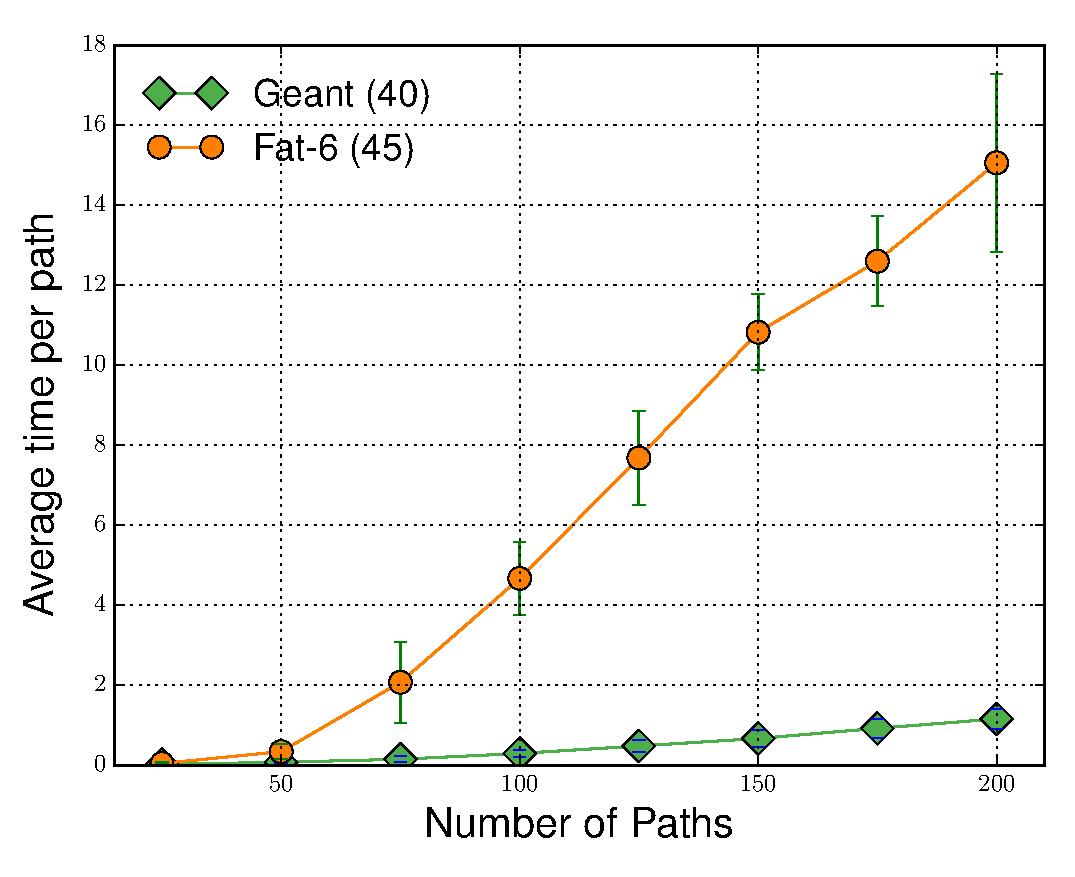
\includegraphics[width=0.66\columnwidth]{figures/ospfTime.eps}}
	\subfloat[Number of Route Filters]
	{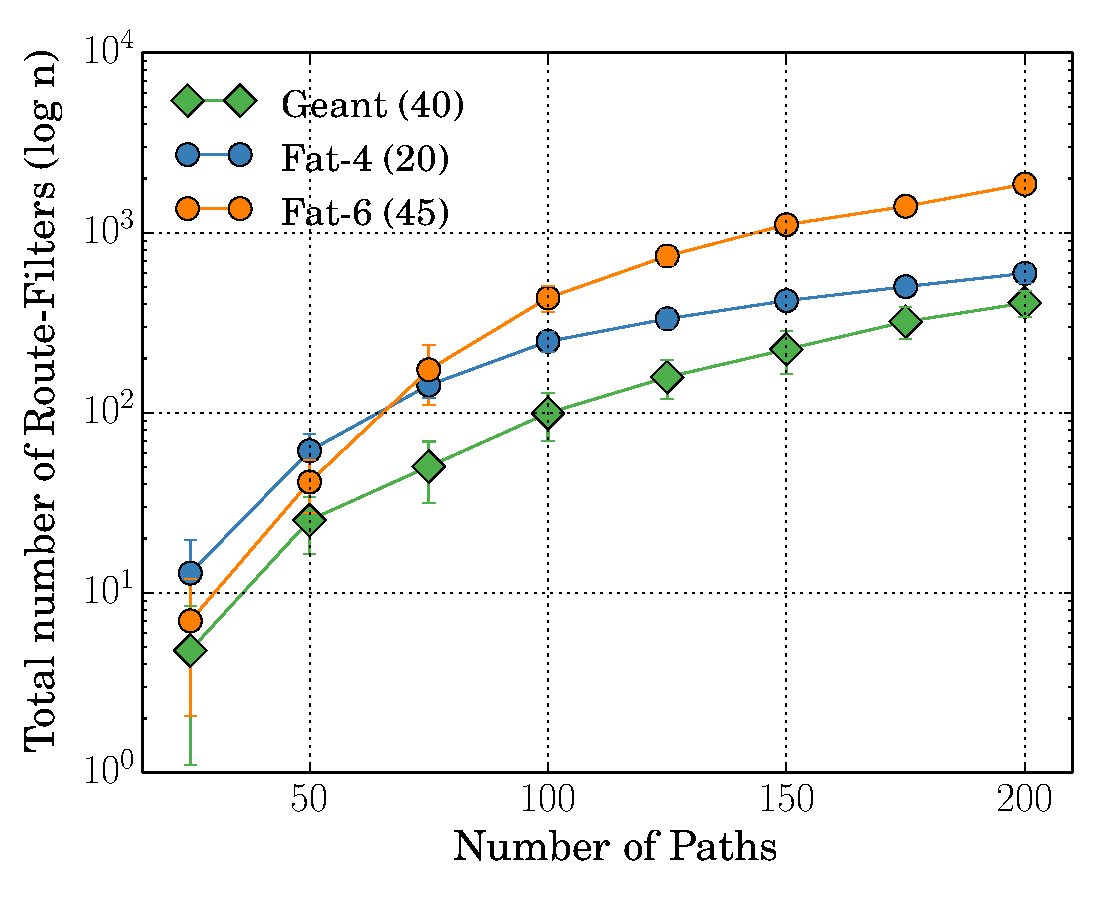
\includegraphics[width=0.66\columnwidth]{figures/ospfRF.eps}}
	\subfloat[Endpoint Resilience]
	{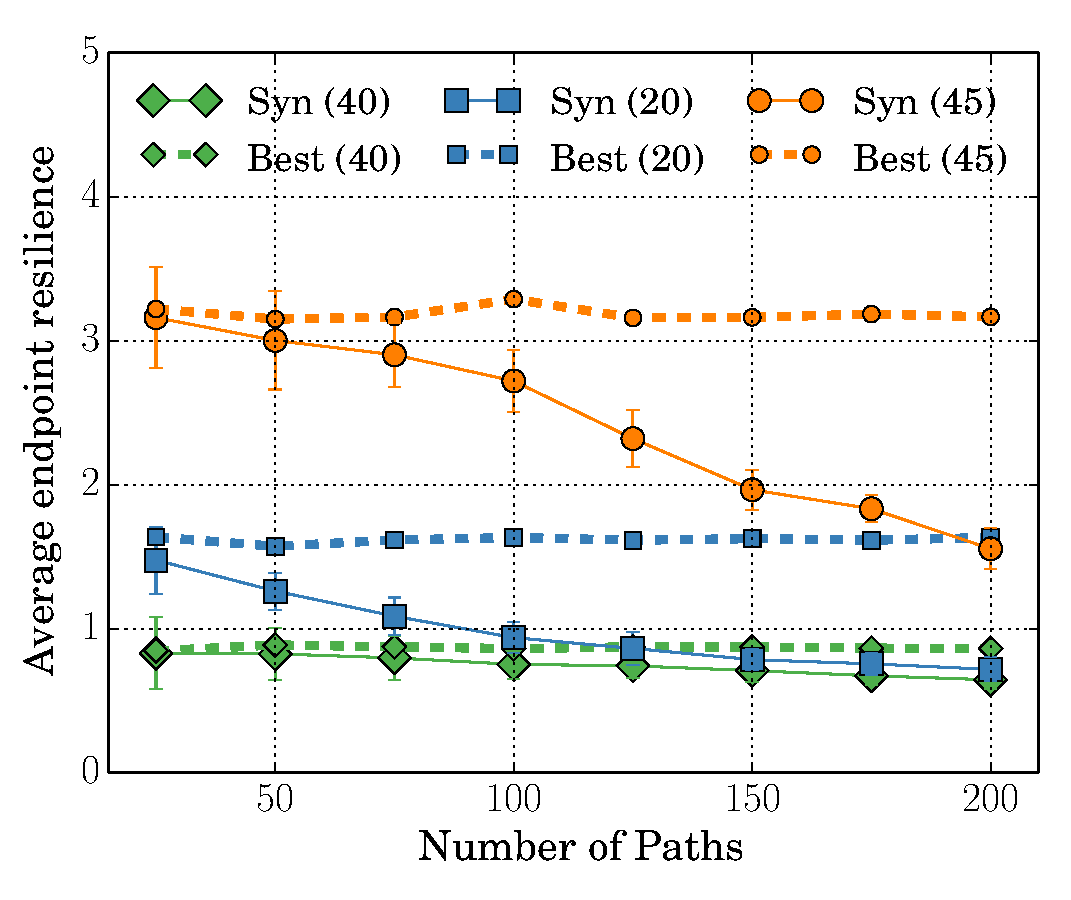
\includegraphics[width=0.65\columnwidth]{figures/ospfAvgRes.eps}}
	\compactcaption{\label{fig:ospfeval}
		OSPF Synthesis evaluation}
\end{figure*}





\section{Evaluation}
 \label{sec:evaluation}
 
 We implemented a prototype of \name in Python. Our prototype uses the
 LP solver Gurobi~\cite{gurobi} for synthesis of OSPF configurations.
 For a given workload, \name outputs abstract configurations, which
 can be translated to actual device configurations using
 templates~\cite{template}.  In this section, we evaluate \Name using
%\loris{really don't like the word realistic}
enterprise-scale data
center fat-tree topologies~\cite{fattree} of different 
sizes, and ISP topologies from the Internet Topology Zoo 
dataset~\cite{zoo}.  
Specifically, we ask:
\begin{itemize}
	\item What is the performance of \Name's algorithm for
          synthesizing OSPF configurations? How do the synthesis time
          and resilience properties vary with size and type of the
          network and number of paths? (\secref{sec:ospfeval})
	
	\item How well does \name's stochastic domain assignment 
	search work in optimizing configuration overhead
	and maximizing endpoint resilience of the paths? (\secref{sec:mcmceval})
	
	\item How does \name perform end-to-end going from policies to
          configurations in conjunction with \genesis?
          (\secref{sec:genzep})
\end{itemize}
All experiments were conducted using a
32-core Intel-Xeon 2.40GHz CPU machine and
128GB of RAM.

\subsection{OSPF Synthesis Performance}
To benchmark the performance of \name's OSPF synthesis,
we consider three topologies: Geant ISP topology with 40 routers,
and 2 fat-tree topologies with 20 (Fat-4) and 45 routers (Fat-6). 
These sizes are consistent with operator preferences to restrict
the size of a domain to under 50 routers (OSPF does not scale
well as domain size increases). We generate $n$ random input paths for
$n/4$ destinations spread across the topology and path
lengths in the range [3, 5]. For each metric, we perform 20 experiments
and report average and standard deviation. 

\noindent\textbf{Synthesis Time.}~~~\Cref{fig:ospfeval}(a) 
shows the synthesis time for increasing number of paths. 
The time taken for Fat-6 is much greater than Fat-4 or Geant
due to have more links; therefore there are more link weights
to synthesize, and greater alternate paths to add constraints for. 
For Geant, we can synthesize weights and filters in 200 seconds 
for 200 paths. Thus OSPF synthesis is effective for ISP topologies
which have fewer links than datacenter topologies.

\Cref{fig:ospfeval}(b) shows the number of filters synthesized. 
As the time taken is dependent on the number of iterations of
the route-filter learning procedure, the number of filters
shows a similar trend to OSPF synthesis time. On average, 2 route-filters
are required for each path in the Geant topology. 

\noindent\textbf{Endpoint Resilience.}~~~\name's OSPF synthesis picks
filters which have the least effect on endpoint resilience, as it  
is a more important metric than the number of filters. We express this
by computing the average of $t-resilience$ for each endpoint considering
the filters ($t-resilience$ means size of mincut is $t+1$).
\Cref{fig:ospfeval}(c) shows the average
endpoint resilience obtained by \name (solid traces) 
compared to the best endpoint resilience (achieved
if there were no filters). For Geant, the endpoint 
resilience obtained by \name trails the best by a small margin,
even though 2 route-filters were required for each path. For
Fat-4 and Fat-6, there is a significant difference between resilience
of the endpoints in \name and the best resilience. 
However, we are able to achieve more than
50 percent of the resilience offered by the topology. 

\begin{figure*}[!t]
	\centering
	\subfloat[Configuration Overhead]
	{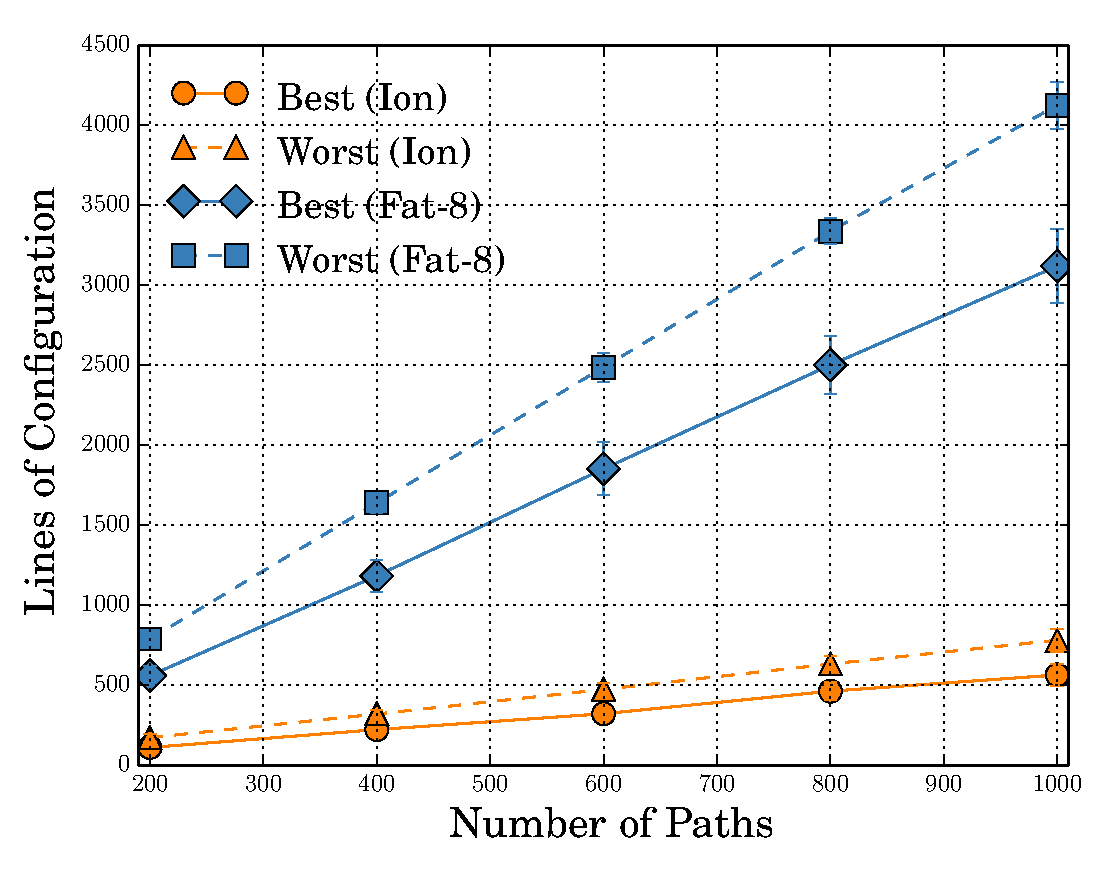
\includegraphics[width=0.66\columnwidth]{figures/confMCMC.eps}}
	\subfloat[Total Loss of Resilience]
	{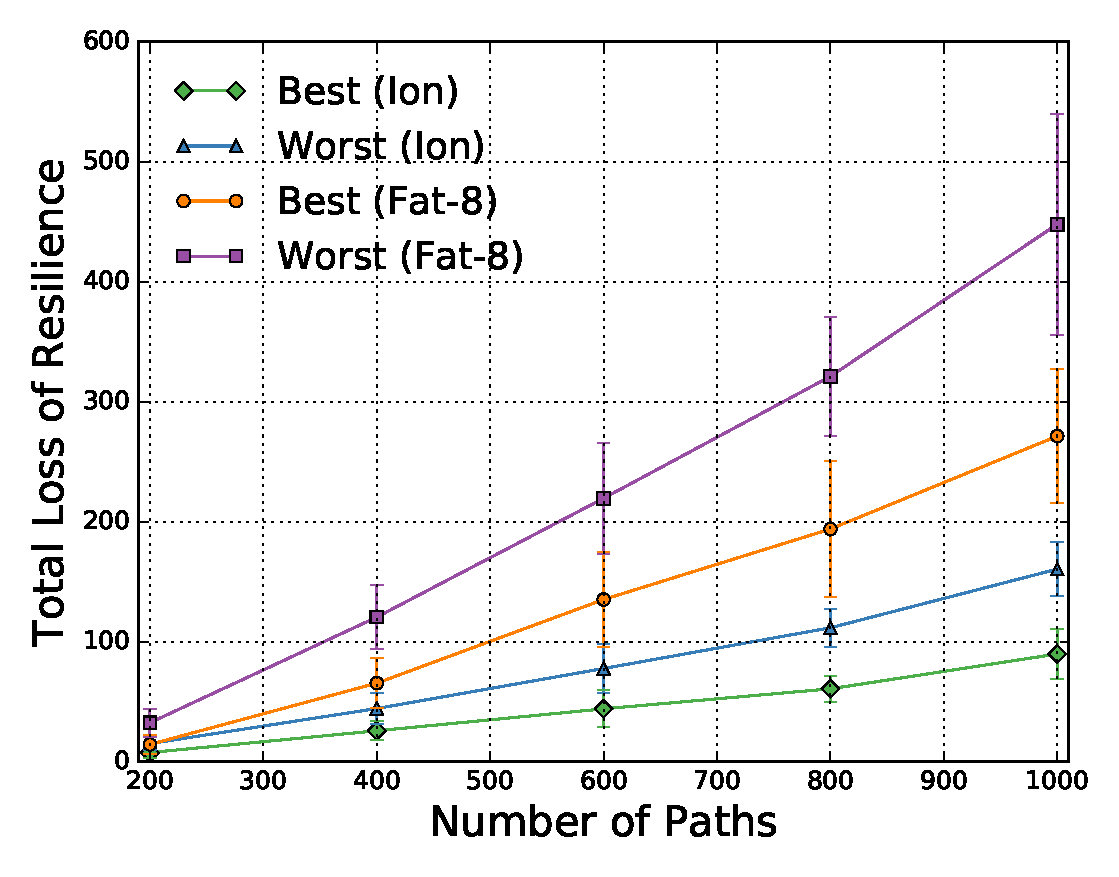
\includegraphics[width=0.66\columnwidth]{figures/TRLMCMC.eps}}
	\subfloat[MCMC Optimizations]
	{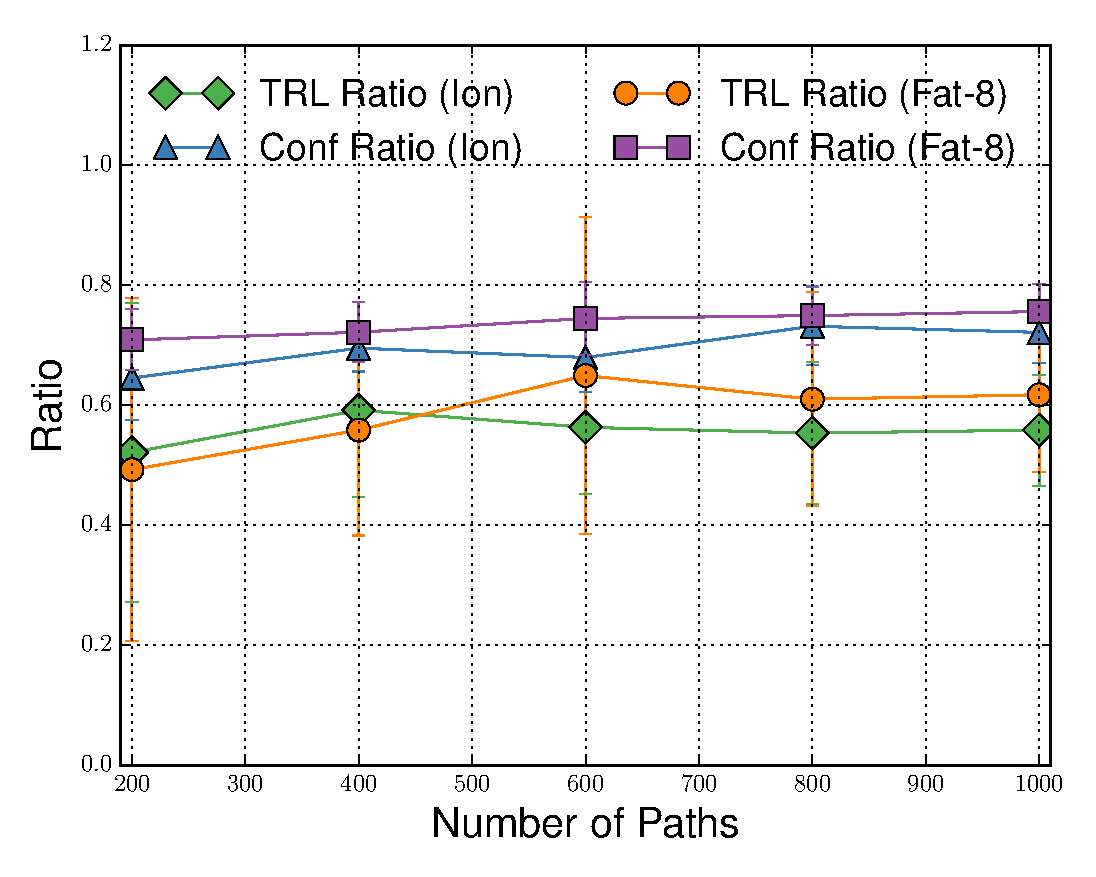
\includegraphics[width=0.66\columnwidth]{figures/ratioMCMC.eps}}
	\compactcaption{\label{fig:mcmceval}
	MCMC Evaluation }
\end{figure*}

\subsection{Dynamic Domain Assignment Performance} \label{sec:mcmceval}
In this section, we demonstrate the advantages of using MCMC sampling
to find a domain assignment which can provide higher endpoint
resilience with lower configuration overhead. For these experiments,
we consider two topologies: the Ion ISP topology (125 routers), and a
80 router fat-tree topology (Fat-8). We run the MCMC sampling for 600s
(iterations $>$ 100,000), and the tunable parameter $\alpha$ assigning
priority for optimizing configuration overhead or route-filters is set
to 1. For the input, we generate random $n$ paths for $n/4$
destination IPs, with path length chosen at random from $[3,10]$. We
split the network into 5 OSPF domains each with size $\in [10,40]$. We
conduct these experiments 20 times each, and report the average and
std. deviation of the metrics.

\noindent\textbf{Configuration Overhead.}~~~
\Cref{fig:mcmceval}(a) shows the configuration overhead $bc + rc$ 
incurred by \name for synthesizing inter-domain configurations.
For the Fat-8 topology which has greater path diversity, we incur more 
overhead to ensure path-compliance than the Ion topology. 
The Best traces indicate the best domain assignment found by MCMC, while 
Worst traces indicates the domain assignment with greatest 
configuration cost. 
This illustrates
the effectiveness of MCMC sampling in finding configurations with lower overhead on average.

\noindent\textbf{Endpoint Resilience.}~~~ \Cref{fig:mcmceval}(b) shows
the loss in total endpoint resilience with varying number of paths
(the count of backup paths for endpoints filtered by the
configurations). For the Worst traces, we store the worst domain
assignment in terms of route-filter cost and synthesize the OSPF
configurations for each domain and calculate the total resilience
loss. We observe that the MCMC sampling can find domain assignments
with lower resilience loss than the worst case. This also illustrates
the effectiveness of the route-filter estimate we use for the cost
function: a reduction in cost results in greater resilience.

\noindent\textbf{Joint Optimization.}~~~
We plot the average Conf Ratio 
(Best configuration overhead/Worst configuration overhead) and TRL
Ratio (Best total loss of resilience/Worst total loss of resilience)
for varying number of paths in \Cref{fig:mcmceval}(c). The MCMC
sampling is able to find a domain assignment
with 1.6$\times$ higher total endpoint resilience for both types
of topologies. At the same time, it is also able to reduce configuration
overhead by a factor of $0.3\times$. The tunable parameter $\alpha$ 
can be used to assign different priorities to these objectives to get
different trends. 

\noindent\textbf{Summary}.
\kausik{Discuss Genesis Experiment}
